% =====================================================================
%  Conpot ICS/SCADA Honeypot — project presentation (LaTeX Beamer)
% ---------------------------------------------------------------------
%  Compile:  pdflatex presentation.tex   (run twice for the outline)
%            or latexmk -pdf presentation.tex
%            or upload this folder to https://overleaf.com and press Compile
%  Figures live in ./figures/ (charts generated from the real conpot.log).
%  TODO: fill in the team names + course on the title slide (marked below).
% =====================================================================
\documentclass[aspectratio=169,11pt]{beamer}

\usetheme{Madrid}
\usecolortheme{whale}
\setbeamertemplate{navigation symbols}{}      % drop the nav clutter
\setbeamertemplate{caption}[numbered]
\setbeamertemplate{frametitle continuation}{}  % no "(cont.)"

\usepackage{graphicx}
\usepackage{booktabs}
\usepackage{xcolor}
\usepackage{tikz}
\usetikzlibrary{arrows.meta,positioning}

\graphicspath{{figures/}}

% --- custom accent colours ---
\definecolor{hpblue}{HTML}{1F4E79}
\definecolor{hpred}{HTML}{C0392B}
\definecolor{hpgreen}{HTML}{1E8449}
\setbeamercolor{structure}{fg=hpblue}
\setbeamercolor{frametitle}{bg=hpblue,fg=white}

\newcommand{\high}{\textcolor{hpred}{\textbf{High}}}
\newcommand{\seq}{scan $\to$ read $\to$ write}

% ---------------------------------------------------------------------
\title[Conpot ICS Honeypot]{Building and Attacking an ICS/SCADA Honeypot}
\subtitle{Conpot over Modbus, SNMP and S7comm --- live attack probes and automated log analysis}

% TODO: replace the bracketed names/course before the viva
\author[Team]{[Your Name] \inst{1} \and Awez [Surname] \inst{1}}
\institute[]{\inst{1}[Course / Module — University]}
\date{\today}

\begin{document}

% ===================== TITLE =====================
\begin{frame}[plain]
  \titlepage
  \begin{center}\small
    \textit{Honeypot \& attacker side} --- [Your Name] \quad\textbullet\quad
    \textit{Log analysis \& dashboard} --- Awez
  \end{center}
\end{frame}

% ===================== OUTLINE =====================
\begin{frame}{Outline}
  \tableofcontents
\end{frame}

% =====================================================================
\section{Background}
% =====================================================================
\begin{frame}{Why an ICS/SCADA honeypot?}
  \begin{itemize}
    \item Industrial Control Systems (ICS/SCADA) run power, water and factory plants
          using legacy protocols --- \textbf{Modbus}, \textbf{S7comm}, \textbf{SNMP} ---
          that were built with \emph{little or no authentication}.
    \item These devices are increasingly reachable from the network, and attackers
          actively scan for them (Shodan, automated ICS worms).
    \item A \textbf{honeypot} is a decoy device: it looks like a real PLC, has no real
          process behind it, and \emph{logs everything an attacker does}.
  \end{itemize}
  \vfill
  \begin{block}{Our goal (two-person project)}
    Stand up a realistic ICS honeypot, attack it ourselves over three protocols, and
    turn the raw honeypot log into structured events, risk scores and a dashboard.
  \end{block}
\end{frame}

\begin{frame}{Conpot --- the honeypot engine}
  \begin{columns}[T]
    \begin{column}{0.58\textwidth}
      \begin{itemize}
        \item Open-source, low-interaction ICS honeypot from the \textbf{Honeynet Project}.
        \item Emulates a \textbf{Siemens SIMATIC S7-200} PLC.
        \item Speaks \textbf{Modbus/TCP}, \textbf{S7comm}, \textbf{SNMP} and \textbf{HTTP}
              on one container.
        \item Answers with believable device identity, so a scanner thinks it found a
              real PLC --- then records the interaction.
      \end{itemize}
    \end{column}
    \begin{column}{0.42\textwidth}
      \begin{block}{Division of work}
        \textbf{Half A} --- deploy Conpot, attack it, capture \texttt{conpot.log}.\\[4pt]
        \textbf{Half B} --- parse the log, detect attack patterns, build a dashboard.
      \end{block}
    \end{column}
  \end{columns}
\end{frame}

% =====================================================================
\section{Architecture}
% =====================================================================
\begin{frame}{System architecture}
  \begin{center}
  
\begin{tikzpicture}[
      box/.style={draw=hpblue,very thick,rounded corners,align=center,
                  fill=hpblue!8,minimum height=1.05cm,font=\footnotesize,inner sep=5pt},
      arr/.style={-{Stealth[length=3mm]},very thick,hpblue}]
    \node[box] (lap)    {Windows laptop\\\textit{Python probes}};
    \node[box,right=1.0cm of lap] (dkr) {Docker Desktop\\publishes to\\\texttt{127.0.0.1}};
    \node[box,right=1.0cm of dkr,fill=hpred!8,draw=hpred] (cp) {\textbf{Conpot}\\Siemens S7-200};
    \draw[arr] (lap) -- (dkr);
    \draw[arr] (dkr) -- (cp);
  \end{tikzpicture}
  \end{center}
  \vfill
  \begin{columns}[T]
    \begin{column}{0.5\textwidth}
      Attacker and honeypot run on one laptop: the Conpot \textbf{Docker} container
      publishes its ICS ports on \texttt{127.0.0.1}, so every probe targets localhost
      and reaches the container directly.
    \end{column}
    \begin{column}{0.5\textwidth}
      \centering
      \begin{tabular}{@{}lcc@{}}
        \toprule
        \textbf{Service} & \textbf{Laptop port} & \textbf{Conpot port}\\
        \midrule
        Modbus      & 502  & 5020  \\
        S7comm      & 102  & 10201 \\
        SNMP (udp)  & 161  & 16100 \\
        HTTP        & 8080 & 8800  \\
        \bottomrule
      \end{tabular}
    \end{column}
  \end{columns}
\end{frame}

% =====================================================================
\section{Attacking the honeypot}
% =====================================================================
\begin{frame}{Attack methodology --- three probes}
  All run from the Windows laptop against \texttt{127.0.0.1}; each is a small Python
  script that generates clean, labelled traffic for the log.
  \vfill
  \begin{columns}[T]
    \begin{column}{0.33\textwidth}
      \begin{block}{Modbus \scriptsize(pymodbus)}
        Read coils, discrete inputs, holding \& input registers; then a
        \textbf{write} to a holding register (value 1234).
      \end{block}
    \end{column}
    \begin{column}{0.33\textwidth}
      \begin{block}{SNMP \scriptsize(pysnmp)}
        \texttt{GET} on system OIDs and a \texttt{WALK} of
        \texttt{1.3.6.1.2.1.1}\\ (v2c, community \texttt{public}).
      \end{block}
    \end{column}
    \begin{column}{0.33\textwidth}
      \begin{block}{S7comm \scriptsize(snap7)}
        Establish an S7 session and request CPU identification (SZL) --- what
        PLCScan does first.
      \end{block}
    \end{column}
  \end{columns}
  \vfill
  \footnotesize The write + multi-protocol scan is deliberate: it is the behaviour of
  a real attacker moving from \emph{reconnaissance} to \emph{tampering}.
\end{frame}

% =====================================================================
\section{Results}
% =====================================================================
\begin{frame}{What the honeypot captured}
  \begin{columns}[c]
    \begin{column}{0.54\textwidth}
      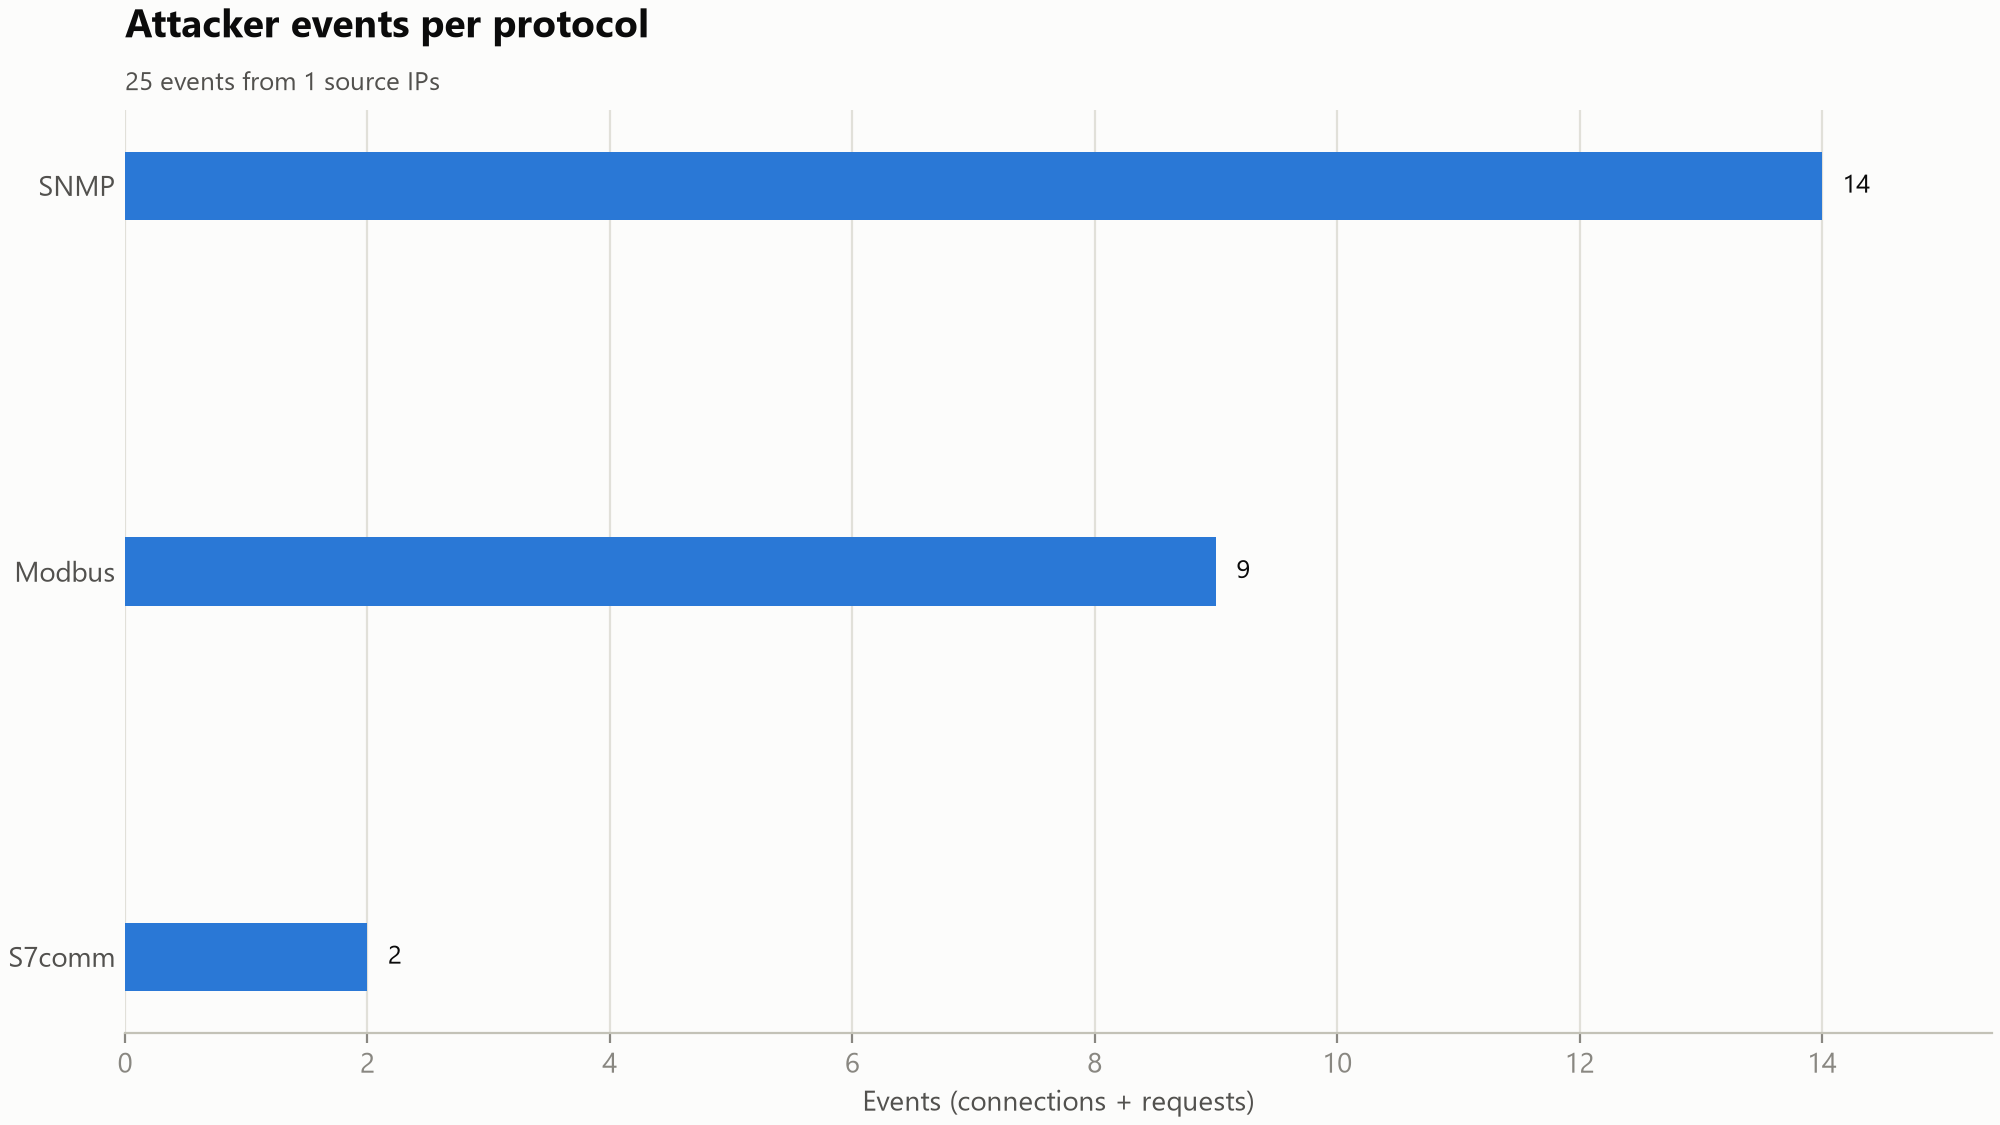
\includegraphics[width=\linewidth]{attacks-per-protocol}
    \end{column}
    \begin{column}{0.46\textwidth}
      \begin{itemize}
        \item \textbf{25 attacker events} from a single source (\texttt{172.17.0.1}, the
              Docker bridge gateway = our laptop).
        \item \textbf{SNMP} dominated (14) --- the full system-tree walk.
        \item \textbf{Modbus} (9): connect, four register reads, one write.
        \item \textbf{S7comm} (2): connection/identification probes.
      \end{itemize}
    \end{column}
  \end{columns}
\end{frame}

\begin{frame}{SNMP recon --- the honeypot \emph{is} a Siemens PLC}
  The SNMP probe returned a convincing fake identity, exactly what an ICS scanner
  looks for:
  \vfill
  \begin{center}
  \begin{tabular}{@{}ll@{}}
    \toprule
    \textbf{OID} & \textbf{Value returned by Conpot}\\
    \midrule
    sysDescr    & Siemens, SIMATIC, S7-200 \\
    sysName     & CP 443-1 EX40 \\
    sysContact  & Siemens AG \\
    sysLocation & Venus \\
    \bottomrule
  \end{tabular}
  \end{center}
  \vfill
  \footnotesize Modbus reads answered with an \texttt{IllegalAddress} exception (the
  stock Conpot template defines no register values) --- the connections and requests
  are still fully logged. The S7 session was established and logged.
\end{frame}

% =====================================================================
\section{Log analysis \& detection}
% =====================================================================
\begin{frame}{From raw log to structured events}
  \begin{columns}[c]
    \begin{column}{0.52\textwidth}
      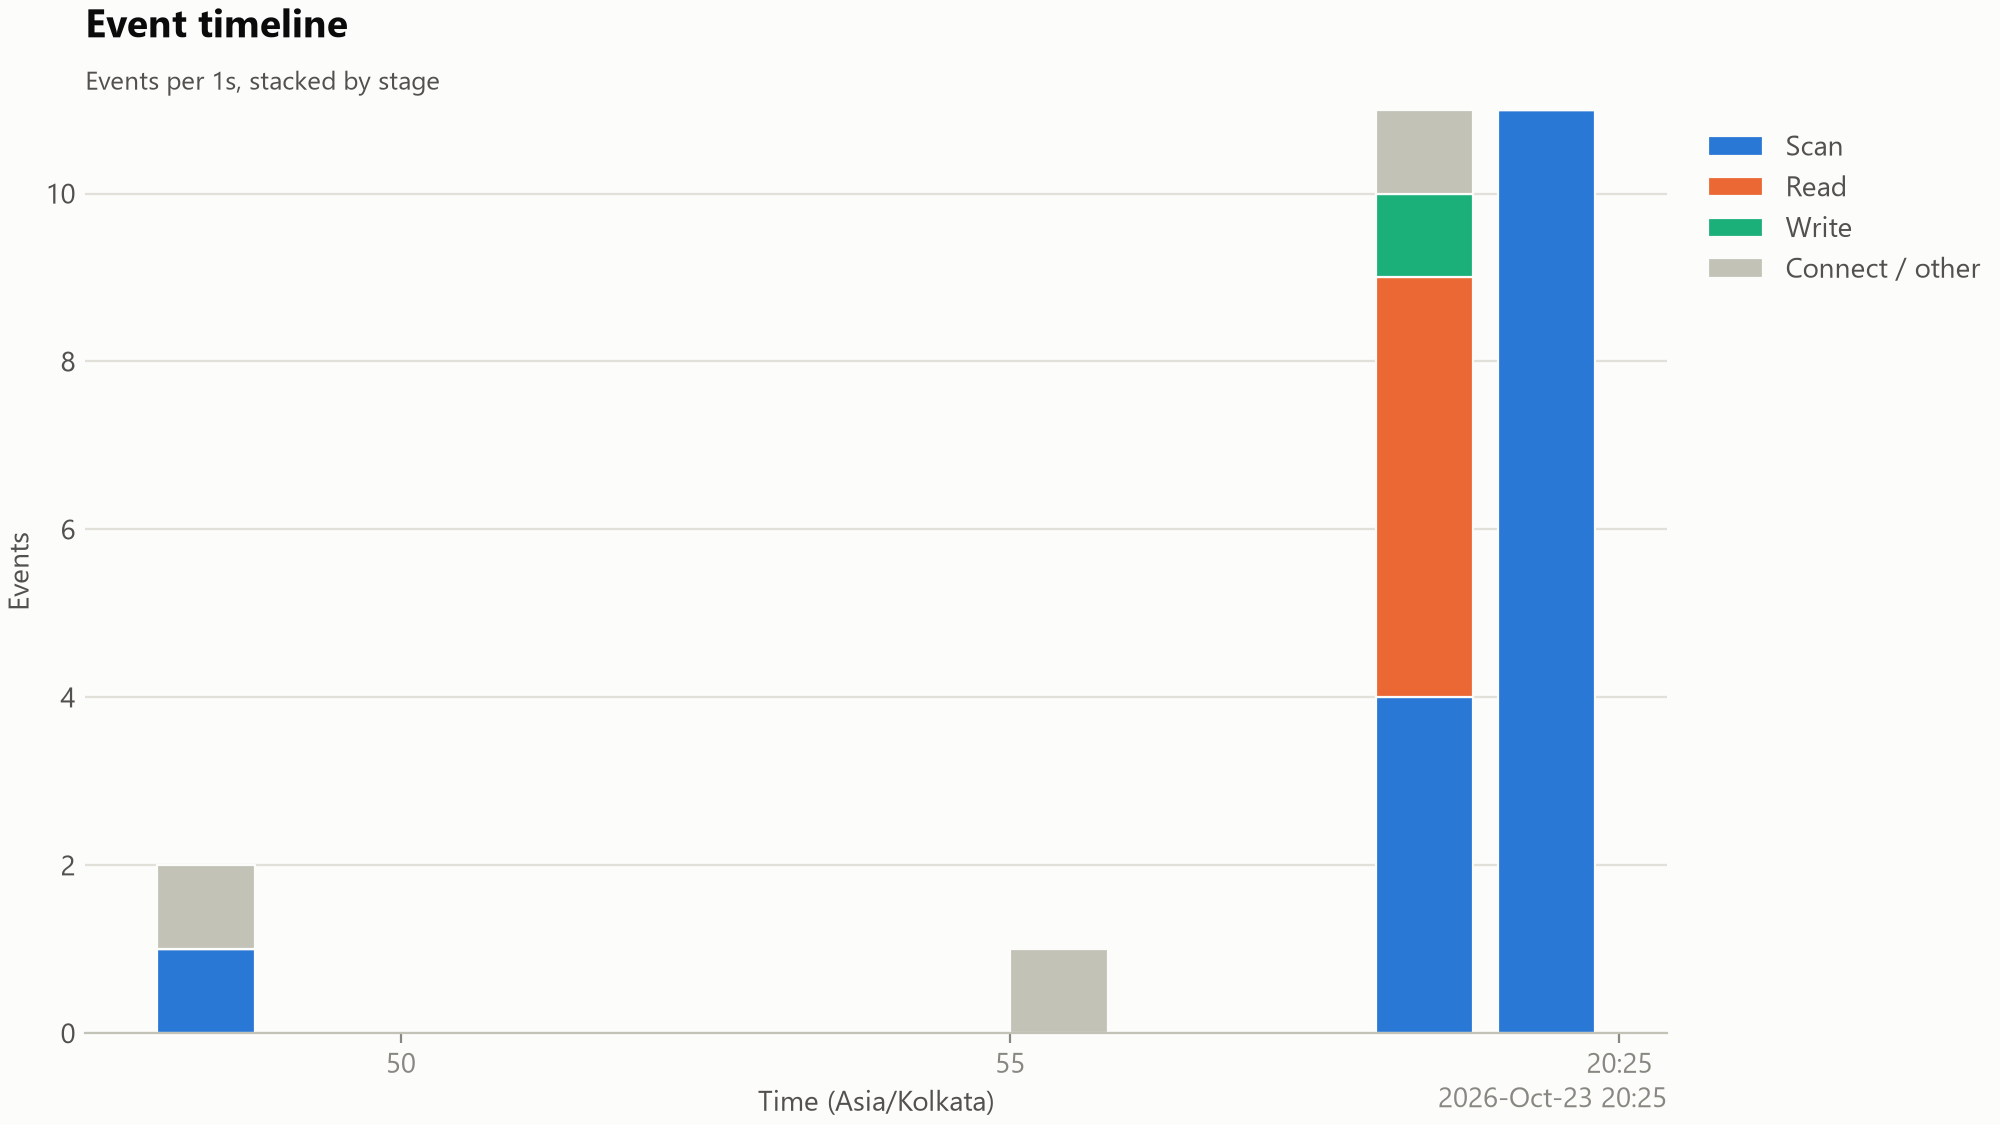
\includegraphics[width=\linewidth]{event-timeline}
    \end{column}
    \begin{column}{0.48\textwidth}
      \textbf{Parser (Half B).} \texttt{conpot.log} $\to$ a pandas table, one row per
      event with:
      \begin{itemize}\footnotesize
        \item protocol, request type, function code
        \item action: \textbf{scan / read / write}
        \item source IP (+ private / Docker-gateway flags)
      \end{itemize}
      131 log lines $\to$ 25 clean events, verified by a \textbf{79-test} suite.
    \end{column}
  \end{columns}
\end{frame}

\begin{frame}{Attack-sequence detection \& risk scoring}
  \begin{columns}[c]
    \begin{column}{0.5\textwidth}
      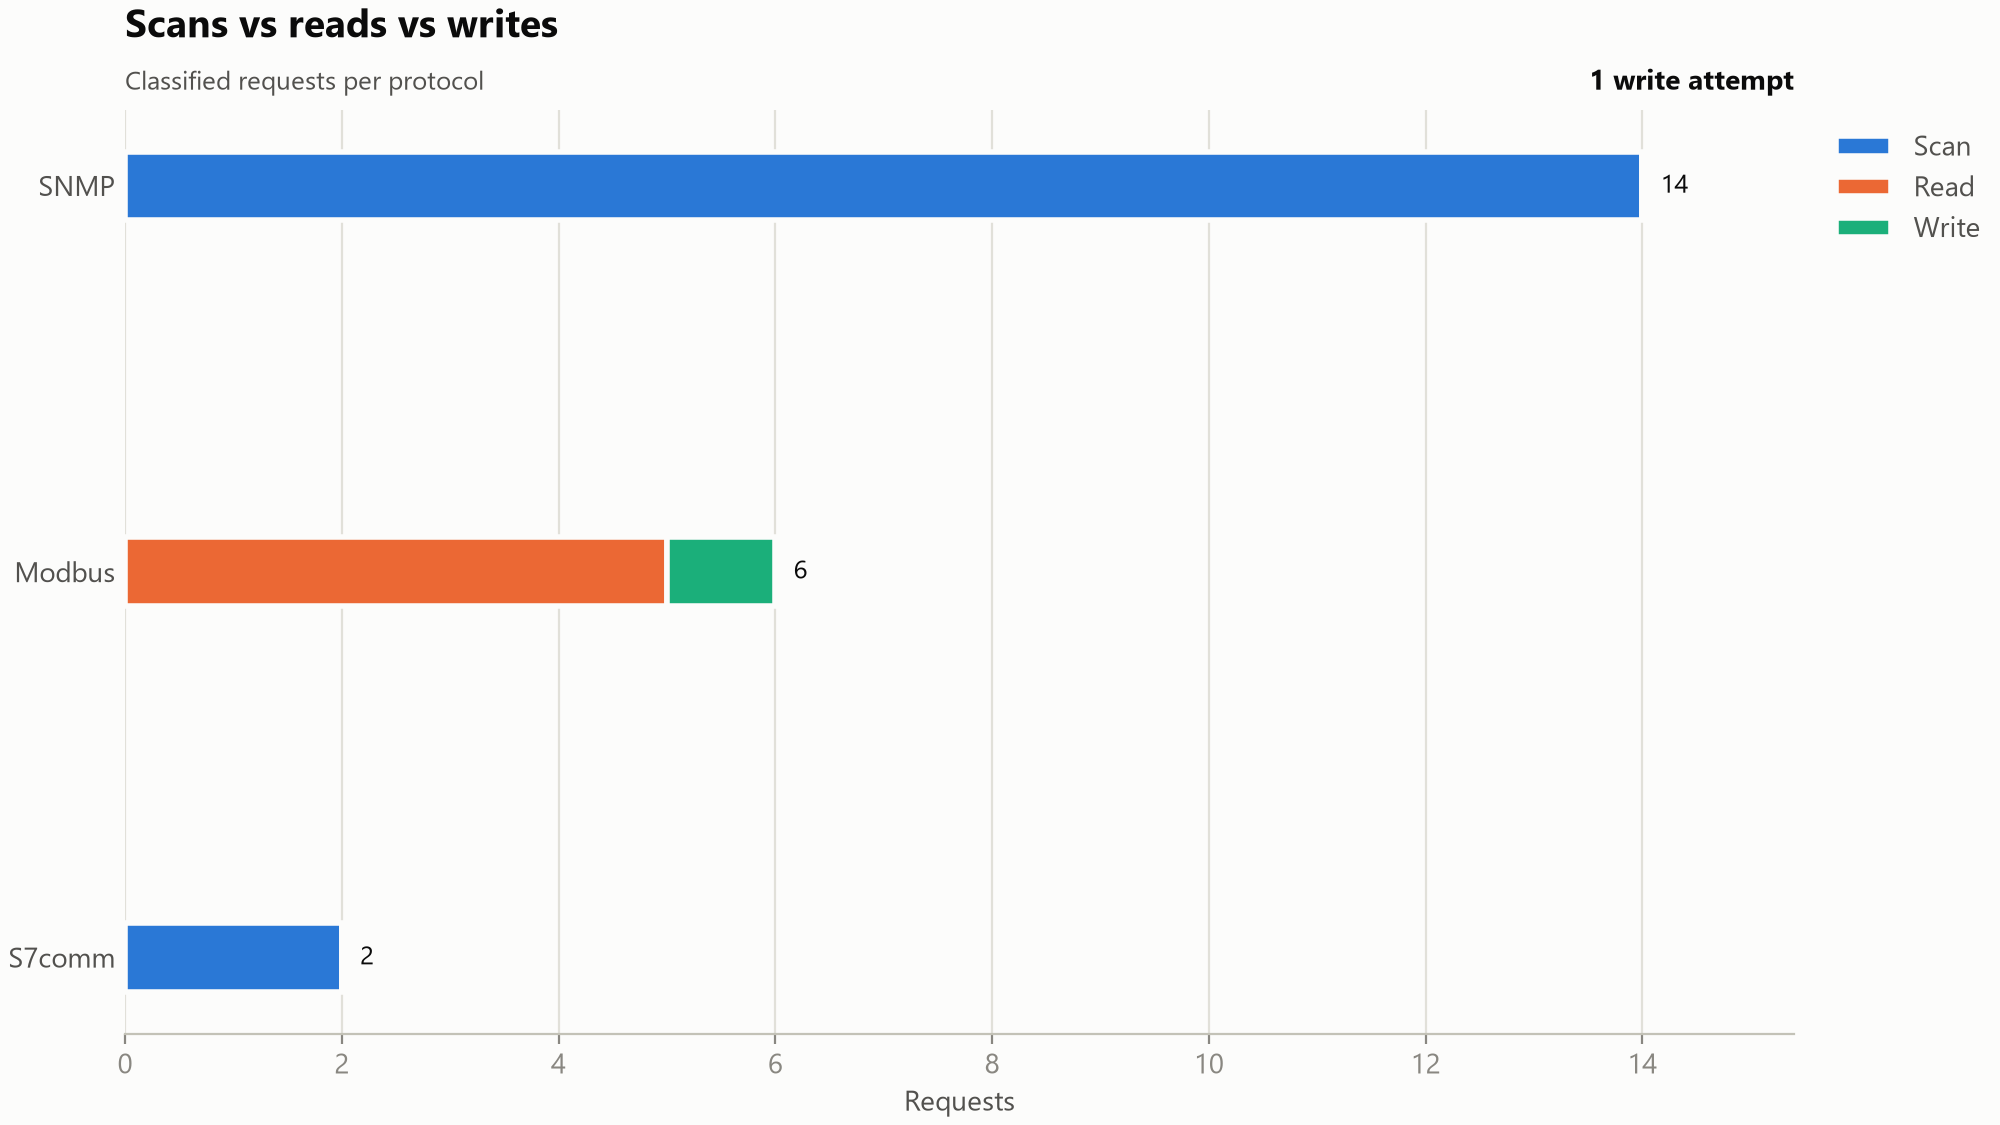
\includegraphics[width=\linewidth]{reads-vs-writes}
    \end{column}
    \begin{column}{0.5\textwidth}
      Per source IP, the detector scores risk from the attack \emph{sequence},
      multi-protocol scanning and any write attempts.
      \vfill
      \begin{block}{Our capture: \texttt{172.17.0.1}}
        Risk: \high\\
        Sequence: \textbf{\seq}\\
        Protocols: modbus, s7comm, snmp\\
        \textcolor{hpred}{Write attempt flagged}
      \end{block}
      \footnotesize The full \seq{} chain across three protocols is the classic
      recon-to-tamper pattern.
    \end{column}
  \end{columns}
\end{frame}

\begin{frame}{Live dashboard}
  \begin{columns}[T]
    \begin{column}{0.55\textwidth}
      A \textbf{Streamlit} dashboard (\texttt{dashboard/app.py}) reads the same log and
      shows, with auto-refresh:
      \begin{itemize}
        \item KPI tiles --- total events, unique source IPs, write attempts.
        \item Risk-by-IP table (Low / Medium / \high).
        \item Protocol mix and gateway share.
      \end{itemize}
      \vfill
      \footnotesize Run with: \texttt{streamlit run dashboard/app.py}
    \end{column}
    \begin{column}{0.45\textwidth}
      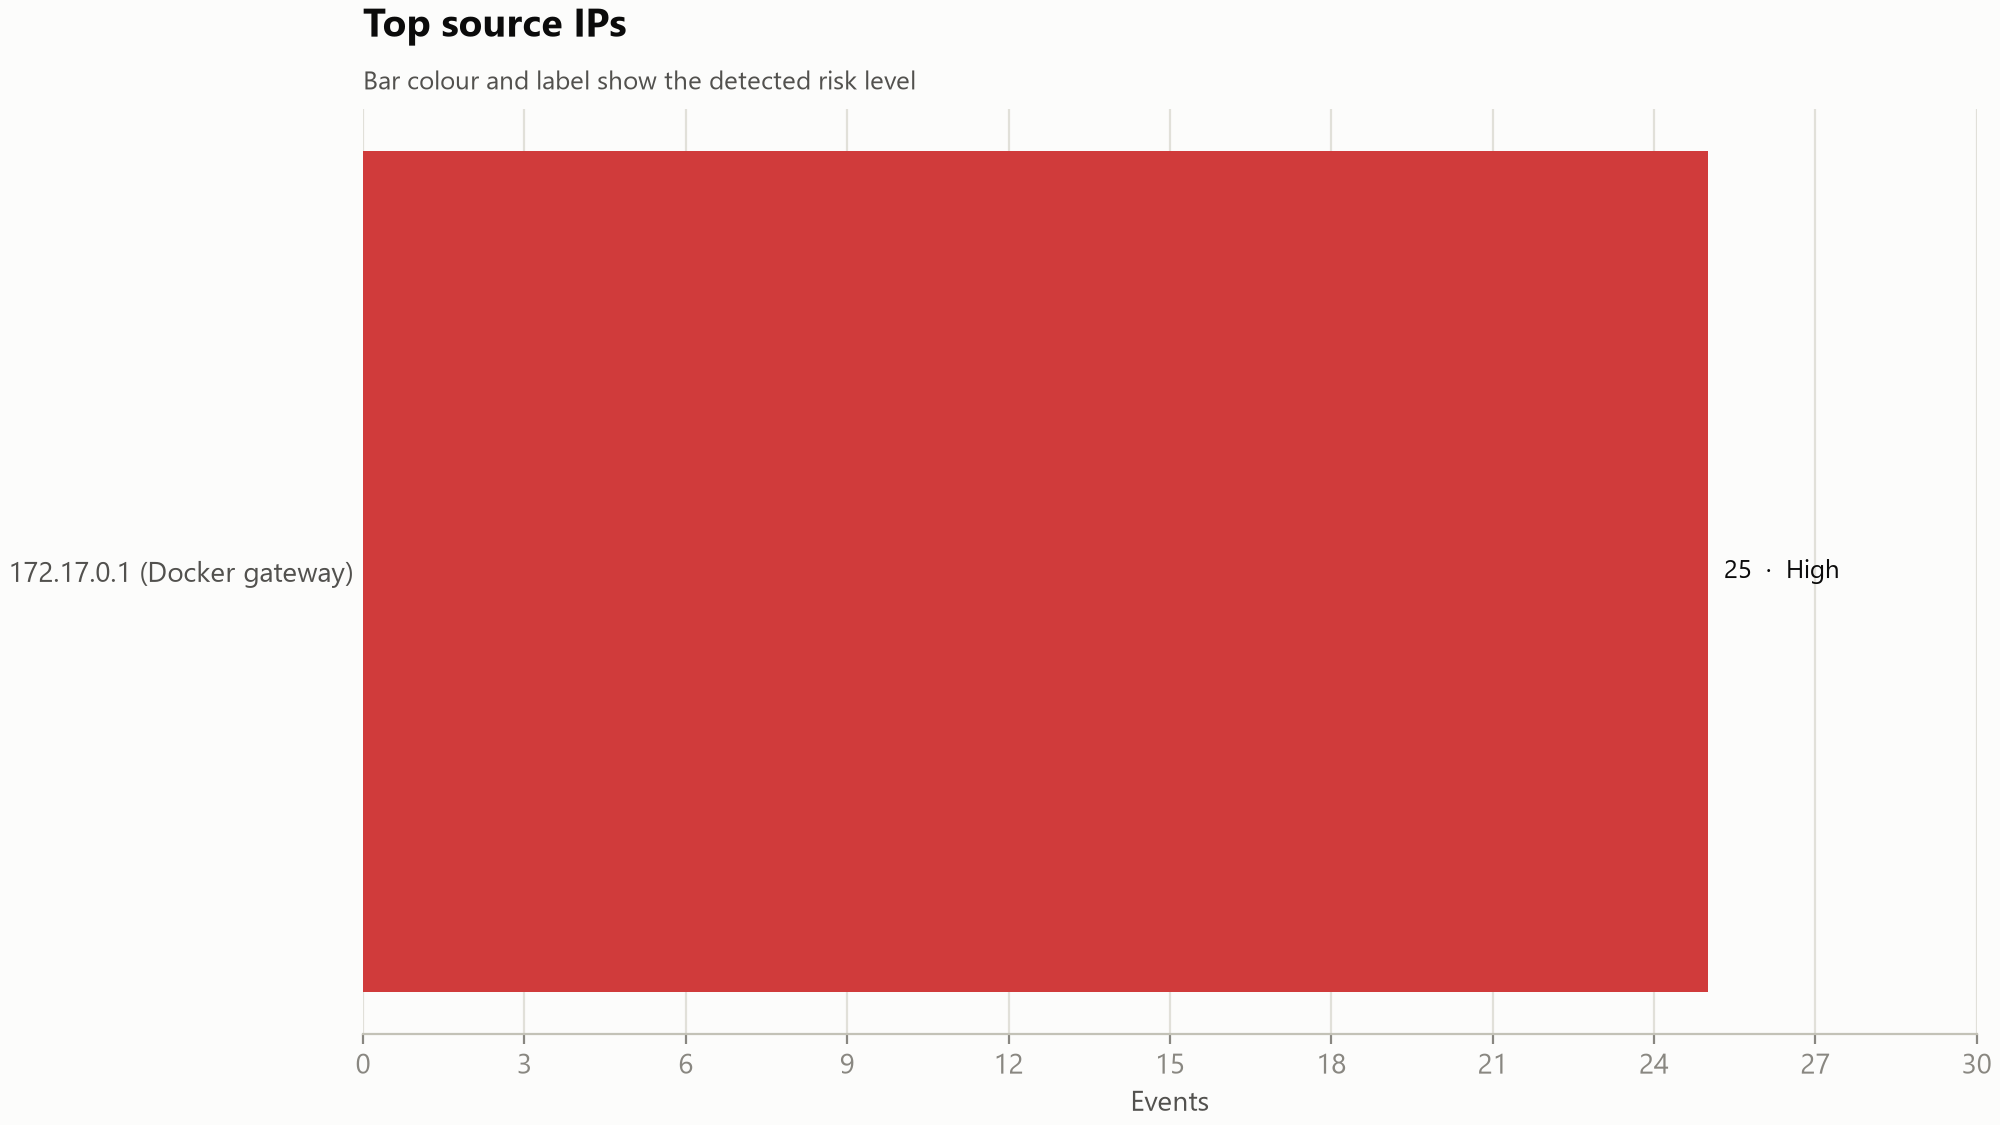
\includegraphics[width=\linewidth]{top-source-ips}
      \begin{center}\footnotesize\textit{Top source IPs (from the real capture)}\end{center}
    \end{column}
  \end{columns}
\end{frame}

% =====================================================================
\section{Wrap-up}
% =====================================================================
\begin{frame}{Ethics \& scope}
  \begin{itemize}
    \item Every probe targets \textbf{our own} honeypot container on \textbf{localhost}
          --- a private, isolated university assignment.
    \item Conpot is purpose-built to be scanned and attacked; no third party is involved.
    \item No tool here is pointed at any host we do not own or have permission to test.
  \end{itemize}
  \vfill
  \begin{block}{Why this is safe and useful}
    The honeypot has no real process to disrupt; the value is entirely in \emph{observing
    and analysing} attacker behaviour in a controlled setting.
  \end{block}
\end{frame}

\begin{frame}{Conclusion \& future work}
  \textbf{What we built}
  \begin{itemize}
    \item A working Conpot ICS honeypot (Siemens S7-200) exercised over Modbus, SNMP and S7comm.
    \item Our own captured attack traffic: 25 events, 3 protocols, scored \high{} risk.
    \item An automated pipeline --- parser, risk detection, charts and a live dashboard
          --- with a 79-test suite.
  \end{itemize}
  \vfill
  \textbf{Future work}
  \begin{itemize}
    \item Expose the honeypot on an isolated public-facing network to capture \emph{real}
          internet scans.
    \item Richer Conpot template (populated registers, more OIDs); add more ICS protocols.
  \end{itemize}
\end{frame}

\begin{frame}[plain]
  \begin{center}
    {\Huge \textcolor{hpblue}{Thank you}}\\[1em]
    {\large Questions?}\\[2em]
    \footnotesize Conpot ICS/SCADA honeypot --- attack \& analysis project
  \end{center}
\end{frame}

\end{document}
